\documentclass[aspectratio=169]{beamer}
\usepackage[utf8]{inputenc}

% design
\usetheme{CambridgeUS}
\usecolortheme{beaver}
\setbeamertemplate{itemize items}[square]
%\setbeamercolor{itemize items}{fg=red}
\usenavigationsymbolstemplate{\beamertemplatenavigationsymbolsempty}

% maths
\usepackage{amsmath, amssymb}
\newcommand{\N}{\mathcal{N}}

% tikz
\usepackage{tikz}
\usetikzlibrary{positioning}

\title[SMC Genealogies]{Asymptotic Genealogies of Sequential Monte Carlo Algorithms}
\author{Suzie Brown}
\date{26 April 2019} 

\begin{document}
\begin{frame}
\maketitle
\end{frame}

\begin{frame}{State space models}
\begin{columns}
\begin{column}{0.45\textwidth}
\begin{align*}
& X_0, \dots, X_T \in \mathcal{X} \\
& Y_0, \dots, Y_T \in \mathcal{Y} \\[12pt]
& X_0 \sim \mu(\cdot) \\
& X_{t+1} \mid (X_t = x_t) \sim f(\cdot | x_t)\\
& Y_t \mid (X_t = x_t) \sim g(\cdot | x_t)
\end{align*}
%%% label each of those (^) lines with initial/transition/emission
\end{column}

\begin{column}{0.45\textwidth}
\begin{center}
\begin{tikzpicture}
\node (yt) {$Y_t$};
\node (thet) [below=of yt] {$X_t$};
\node (yt1) [left=of yt] {$Y_{t-1}$};
\node (thet1) [below=of yt1] {$X_{t-1}$};
\node (dot1) [left=of thet1] {$\dots$};
\node (dot2) [right=of thet] {$\dots$};
\draw[->](thet.north)--(yt.south) node[midway, right] {\footnotesize{$g$}};
\draw[->](thet1.north)--(yt1.south) node[midway, right] {\footnotesize{$g$}};
\draw[->](thet1.east)--(thet.west) node[midway, above] {\footnotesize{$f$}};
\draw[->](dot1.east)--(thet1.west) node[midway, above] {\footnotesize{$f$}};
\draw[->](thet.east)--(dot2.west) node[midway, above] {\footnotesize{$f$}};
\end{tikzpicture}
\end{center}
\end{column}
\end{columns}
\end{frame}

\begin{frame}{Target tracking}
\begin{columns}
\begin{column}{0.6\textwidth}
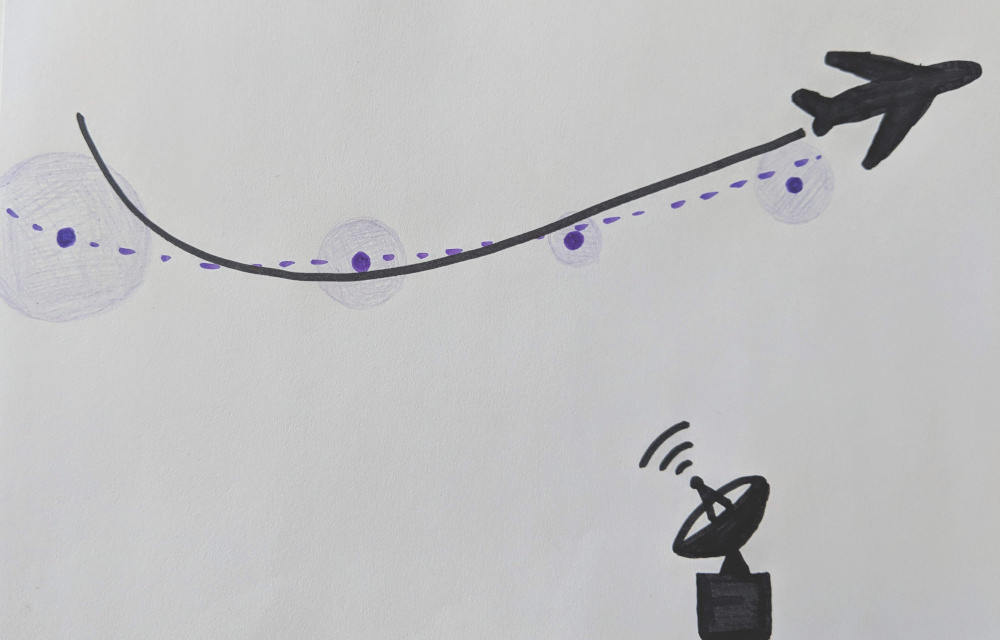
\includegraphics[width=\textwidth]{../tracking.jpg}
\end{column}
\begin{column}{0.35\textwidth}
use noisy radar data to infer position/trajectory of aircraft:
\begin{itemize}
\item $f$ models how aircraft moves
\item $g$ models uncertainty in radar measurements
\end{itemize}
\end{column}
\end{columns}
\end{frame}

\begin{frame}{Inference problems}
\textbf{Filtering:} where is it now? $p(x_{t} | y_{0:t})$\\[7pt]
\textbf{Prediction:} where will it go next? $p(x_{t+1} | y_{0:t})$\\[7pt]
\textbf{Smoothing:} where has it been? $p(x_{0:t} | y_{0:t})$\\[12pt]

Smoothing is ``harder'' than filtering/prediction. 
\end{frame}

\begin{frame}{Deterministic solutions}
\begin{columns}
\begin{column}{0.45\textwidth}
{\Large Kalman filter}\\
Under a linear Gaussian model:
\begin{align*}
& X_0 \sim \N(0, \Sigma_0) \\
& X_{t+1} \mid (X_t = x_t) \sim \N(A x_t, \Sigma_x) \\
& Y_t \mid (X_t = x_t) \sim \N(B x_t, \Sigma_y)
\end{align*}
we can recursively compute filtering distributions. 
Then a backward pass of RTS smoother provides smoothing distributions.\\[7pt]
This class of models is rather restrictive.
\end{column}
%\pause
\begin{column}{0.45\textwidth}
{\Large Extended Kalman filter}\\
In non-linear Gaussian models, use a local linear approximation and apply Kalman filter.\\[7pt]
This requires gradients and performs poorly in models that are very non-linear.\\[12pt]
%\pause
{\Large Unscented Kalman filter}\\
For highly non-linear Gaussian models, replace the transition step of Kalman filter by propagating a representative set of points through $f$.
\end{column}
\end{columns}
\end{frame}

\begin{frame}{Deterministic solutions}
\begin{itemize}
\item Kalman filter provides optimal filter for linear Gaussian models, but extended/unscented Kalman filter are no longer optimal.\\[7pt] %%% what does optimal even mean?
\item All of these methods require model to be Gaussian.
Deterministic solutions are available for some other conjugate families, but these are still restrictive. \\[7pt]
\item Solutions are also available in the case that $\mathcal{X}$ is finite (integrals become sums), but we will generally consider $\mathcal{X}$ to be a continuous space. \\[7pt]
\end{itemize}
%\pause
Sequential Monte Carlo (SMC) provides general-purpose (stochastic) methods that do not require a tractable model. Only requires sampling from $f(\cdot | x)$, and pointwise evaluation of $g(y | x)$ up to a normalising constant for each $y$.
\end{frame}

\begin{frame}{Sequential Monte Carlo}
\textbf{Prior: }
$p(x_{0:t}) = \mu(x_0) \prod_{i=1}^t f(x_i | x_{i-1})$ \\[7pt]
\textbf{Likelihood: }
$p(y_{0:t} | x_{0:t}) = \prod_{i=0}^t g(y_i | x_i)$ \\[7pt]
\textbf{Posterior: }
$p(x_{0:t} | y_{0:t}) \propto \mu(x_0) g(y_0 | x_0) \prod_{i=1}^t f(x_i | x_{i-1}) g(y_i | x_i)$\\[12pt]
\begin{itemize}
\item Represent posterior distribution at time $t$ with $N$ particles.\\[7pt]
\item Posterior factorises sequentially --- avoid increase of dimension with $T$.
\end{itemize}
\end{frame}

\begin{frame}{Sequential Monte Carlo}

{\Large Algorithm}\\
After initialisation, iterate these steps:
\begin{itemize}
\item \textbf{Propagate:} move the particles through the transition $f$
\item \textbf{Calculate weights:} weight each particle according to $g$
\item \textbf{Resample:} duplicate high-weight particles and kill off low-weight ones \\[12pt]
\end{itemize}
%\pause
Approximate posterior distribution $p(x_{0:t} | y_{0:t})$ by the empirical measure of the particles:
\begin{equation*}
\hat{p}(x_{0:t}|y_{0:t}) = \frac{1}{N} \sum_{i=1}^N \delta_{X_{0:t}^{(i)}} (x_{0:t})
\end{equation*}
\end{frame}

\begin{frame}{Ancestral degeneracy}
\begin{columns}
\begin{column}{0.6\textwidth}
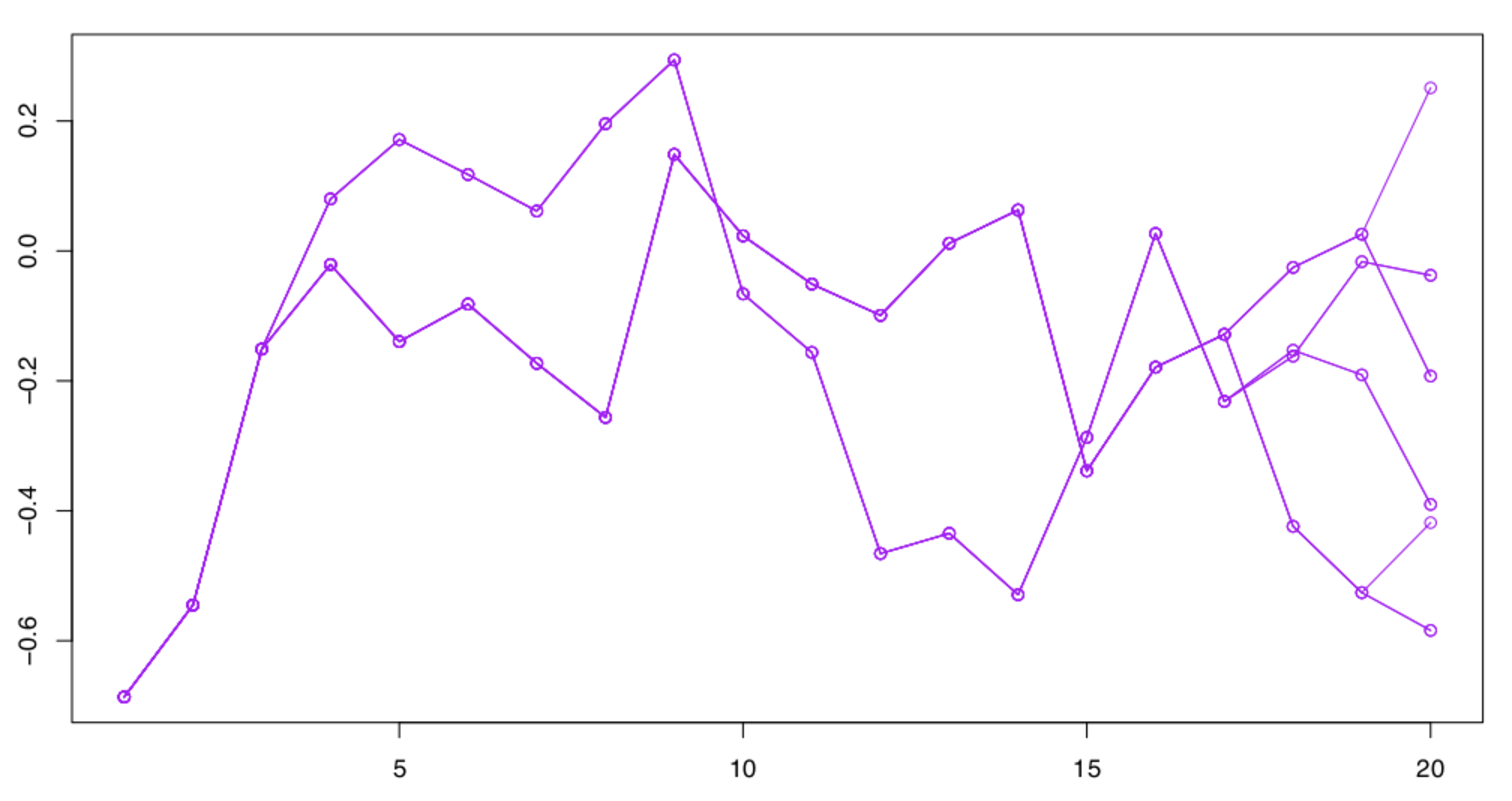
\includegraphics[width=\textwidth]{../degeneracy.pdf}
\end{column}
\begin{column}{0.35\textwidth}
For smoothing we need a sample of trajectories.\\[7pt]
Resampling means that trajectories of time $T$ particles coalesce backwards in time.
\end{column}
\end{columns}
\end{frame}

\end{document}